
\documentclass{article}

%%%%%%%%%%%%%%%%%%%%%%%%%%%%%%%%%%%%%%%%%%%%%%%%%%%%%%%%%%%%%%%%
\usepackage[utf8]{inputenc}
\usepackage[top=3cm, bottom=3cm, left=2.5cm, right=2.5cm]{geometry}
\usepackage{graphicx}
\usepackage{float}
\usepackage[colorlinks=true, linkcolor=blue]{hyperref}
\usepackage{amsmath,amsthm,amsfonts,amssymb}
\usepackage{wrapfig}

\usepackage{Sweave}
\begin{document}
%%%%%%%%%%%%%%%%%%%%%%%%%%%%%%%%%%%%%%%%%%%%%%%%%%%%%%%%%%%%%%%%
  
  
\Sconcordance{concordance:p1.tex:p1.Rnw:%
1 12 1 1 0 1 1 1 19 56 1 1 19 1 2 1 0 2 1 1 5 7 0 1 2 1 1 1 5 1 2 6 1 1 %
2 1 0 2 1 1 5 8 0 1 3 1 1 1 5 1 2 6 1 1 2 1 0 2 1 1 7 5 0 1 7 5 0 1 7 9 %
0 1 3 2 1 1 5 1 2 11 1}


%%%%%%%%%%%%%%%%%%%%%%%%%%%%%%%%%%%%%%%%%%%%%%%%%%%%%%%%%%%%%%%%
  % strona tytulowa
\title{Statistical packages - report 2}
\author{Urszula Grochocińska, Marcin Mazurkiewicz}
\maketitle
\tableofcontents 


%%%%%%%%%%%%%%%%%%%%%%%%%%%%%%%%
  \section{Introduction}
This report concerns checking the hypothesis using three tests: Student t-test, Welch t-test, and Wilcoxon test. In our case the hypothesis is two-sided (we are testing if means of two samples are equal).
  \subsection{Student t-test}
In our case, the test is used for testing hypothesis about mean with equal variances in the samples and with the normal distribution. The test is based on $t$ distribution and the significance level. The $t$ distribution is specified by a number of freedom degrees. With an increasing number of freedom degrees, this distribution converges to the normal distribution.

  The t-test has assumption: independent observations, normal distribution of samples and equal variances for samples. The last one could be dropped if the sample size is large enough.
  In the test we calculate the statistics $t$:
  \begin{equation}
  t=\frac{\overline{x}_1-\overline{x}_2}{\sqrt{s^2\left(\frac{1}{n_1}+\frac{1}{n_2}\right)}},
  \end{equation}
where $\overline{x}_1$ and $\overline{x}_2$ are means, $n_1$ and $n_2$ are sample sizes and $s^2$ is calculated by formula:
  \begin{equation}
    s^2=\frac{\sum_{i=1}^{n_1}(x_i-\overline{x}_1)^2+\sum_{j=1}^{n_2}(x_j-\overline{x}_2)^2}{n_1+n_2-2}.
  \end{equation}
Because of the fact that we have two-sided test we reject the null hypothesis in favor of the alternative if the $t$ statistics is not in the interval $[t_{\alpha/2}, t_{1-\alpha/2}]$. The interval is based on $t$ distribution with $n_1+n_2-2$ number of freedom degrees.

  \subsection{Welch t-test}
This test is an extension of Student t-test. Because of the fact that Student t-test has an assumption about equal variances and normality there appear a need to construct a test to examin a case with unequal variances. Such test is, for example, Welch t-test. There is used a statistic $t$ which is given by the following formula:
  \begin{equation}
     d=\dfrac{\bar{x}_1-\bar{x}_2}{\sqrt{\frac{s_1^2}{n_1}+\frac{s_2^2}{n_2}}},
  \end{equation}
where 
  \begin{equation}
     s_1^2=\dfrac{\sum\limits_{i=1}^{n_1}(x_i-\bar{x}_1)^2}{n_1-1},\, s_2^2=\dfrac{\sum\limits_{i=1}^{n_2}(x_j-\bar{x}_2)^2}{n_2-1}.
  \end{equation}

The number of freedom degrees are given by:
  \begin{equation}
     df=\dfrac{\left[\frac{s_1^2}{n_1}+\frac{s_2^2}{n_2}\right]^2}{\frac{(s_1^2/n_1)^2}{n_1-1}+\frac{(s_2^2/n_2)^2}{n_2-1}}.
  \end{equation}
  
The rest part of the procedure (rejecting or not the null hypothesis) is like Student t-test.

  \subsection{Wilcoxon test}
The last test taken into consideration is the Wilcoxon test. It can be used as a substitution of Student t-test when the distribution of samples is not normal. This test is non-parametric and is used to compare two related samples.

  The algorithm consists of a few steps. Firstly we calculate the differences between pairs of observations $|x_i-y_i|$. Separately we calculate sign of these differences. Then we rank those differences and denote then $R_i$. Statistic $W^+$ is defined as sum of ranks $R_i$ in which the difference $d_i<0$. After all the statistics are compared with the reference table. This comparison results in rejecting or not the hypothesis.


%%%%%%%%%%%%%%%%%%%%%%%%%%%%%%%
  \section{Task 1.}
In the first task we consider two samples of 200 observations in each which have normal distribution with standard deviation $\sigma=2$.
  Firstly we make the function for calculation power function for Student t-test and Wilcoxon test.
 
After that, we use this function and plot power functions for all three test.
\begin{Schunk}
\begin{Sinput}
>   powers_student <- vector(mode="numeric", length=0)
>   powers_welch <- vector(mode="numeric", length=0)
>   powers_wilcoxon <- vector(mode="numeric", length=0)
>   for (i in seq(-2,2,.1)){
+     powers_student = c(powers_student, t.power1(means = c(0, i), sds = c(2,2)))
+     powers_welch = c(powers_welch, t.power1(means = c(0, i), sds = c(2,2), var.equal = FALSE))
+     powers_wilcoxon = c(powers_wilcoxon, wilcoxon.power(means = c(0, i), sds = c(2,2)))
+   }
\end{Sinput}
\end{Schunk}
\begin{figure}
\center
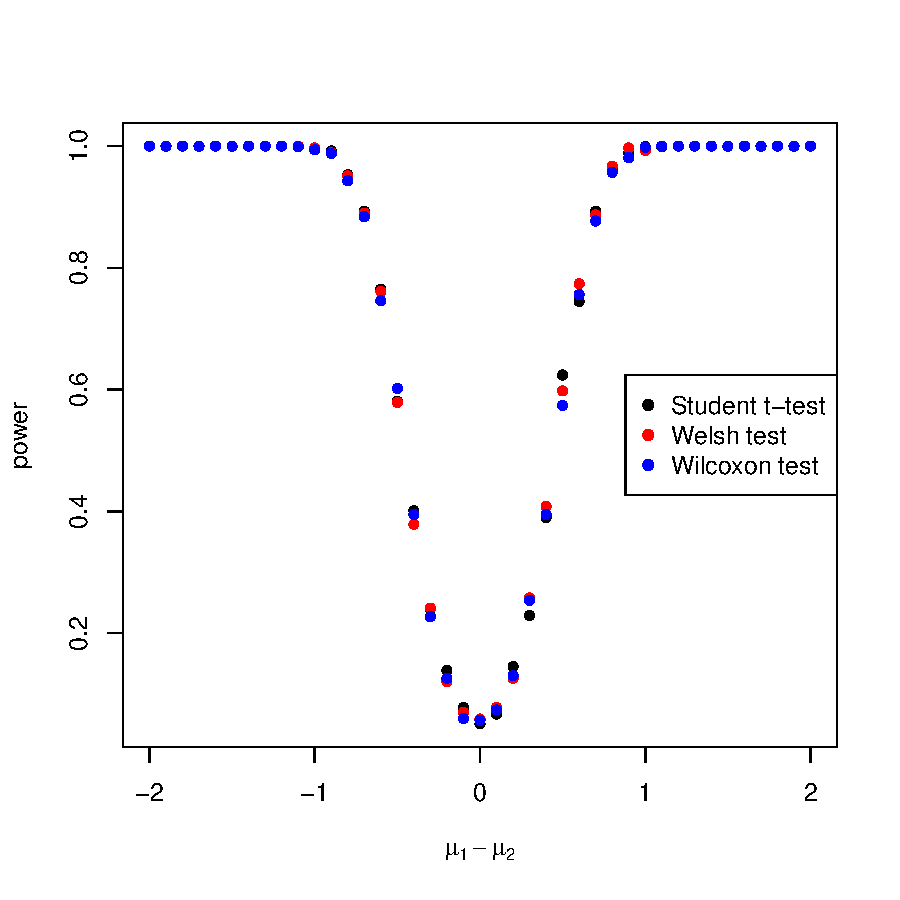
\includegraphics{p1-task_1_plot}
\label{chart_t1}
\caption{Power functions of three tests. Tests for two samples with normal distribution and equal variances.}
\end{figure}
On the first plot \ref{chart_t1} we can see that the power function looks almost the same for all tests when we consider the samples with normal distribution and equal variance. It is also shown that those tests are much more efficient when the difference between means $\mu_1-\mu_2$ is not close to 0. The power function is symmetric and the values decrease significantly faster in $[-1, 1]$ interval of $\mu_1-\mu_2$. Concerning chosen significance level $\alpha=0.05$, there is no uniformly strongest test.

  \section{Task 2.}
 The second task is similar to first but instead of equal variances, we have two samples, one with $\sigma=2$ and the second sample with $\sigma=4$.
\begin{Schunk}
\begin{Sinput}
>   powers_student <- vector(mode="numeric", length=0)
>   powers_welch <- vector(mode="numeric", length=0)
>   powers_wilcoxon <- vector(mode="numeric", length=0)
>   for (i in seq(-2,2,.1)){
+     powers_student = c(powers_student, t.power1(means = c(0, i), sds = c(2,4)))
+     powers_welch = c(powers_welch, t.power1(means = c(0, i), sds = c(2,4), var.equal = FALSE))
+     powers_wilcoxon = c(powers_wilcoxon, wilcoxon.power(means = c(0, i), sds = c(2,4)))
+   }
> 
\end{Sinput}
\end{Schunk}
\begin{figure}
\center
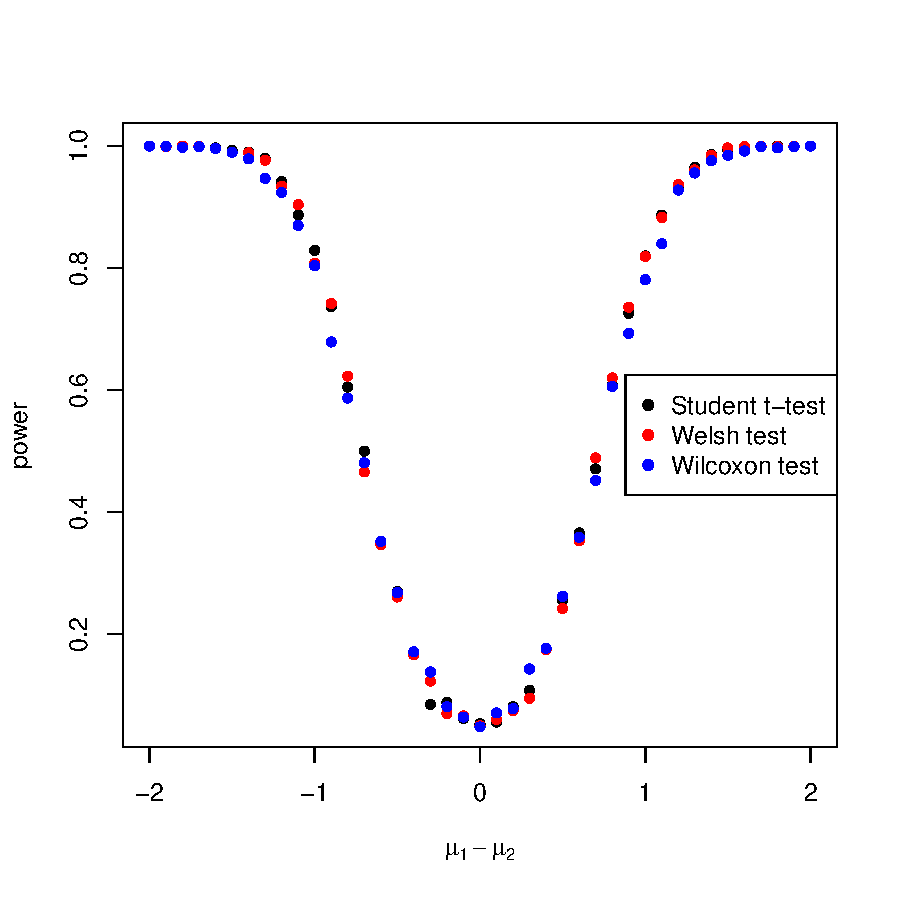
\includegraphics{p1-task_2_plot}
\label{chart_t2}
\caption{Power functions of three tests. Tests for two samples with normal distribution and non equal variances.}
\end{figure}
In the second case, the Student t-test does not meet the assumption about variance equality. In this case, we would like to drop this assumption to see the result. Also, in this case, the differences between test are very small. Comparing the plots \ref{chart_t1} and \ref{chart_t2} we could see that the slope of the curves are different. In first figure, the values decrease faster than in the second chart. Besides the values of power function on the figure \ref{chart_t2} begin to decrease when the difference $|\mu_1-\mu_2|$ is greater than 1.

  \section{Task 3.}
 The last task concerns the case in which the distribution of samples are exponential. 
\begin{Schunk}
\begin{Sinput}
>   powers_student <- vector(mode="numeric", length=0)
>   powers_welch <- vector(mode="numeric", length=0)
>   powers_wilcoxon <- vector(mode="numeric", length=0)
>   for (i in seq(0,4,.1)){
+     tps = replicate(1000,
+                     t.test(rexp(200,rate = 1/2),
+                            rexp(200,rate = 1/i), var.equal = TRUE)$p.value)
+     powers_student = c(powers_student, sum(tps < alpha/2 | tps > 1 - alpha/2) / 1000)
+   }
>   for (i in seq(0,4,.1)){
+     tps = replicate(1000,
+                     t.test(rexp(200,rate = 1/2),
+                            rexp(200,rate = 1/i), var.equal = FALSE)$p.value)
+     powers_welch = c(powers_welch, sum(tps < alpha/2 | tps > 1 - alpha/2) / 1000)
+   }
>   for (i in seq(0,4,.1)){
+     tps = replicate(1000,
+                     wilcox.test(rexp(200,rate = 1/2),
+                                 rexp(200,rate = 1/i))$p.value)
+     powers_wilcoxon = c(powers_wilcoxon, sum(tps < alpha/2 | tps > 1 - alpha/2) / 1000)
+   }
> 
\end{Sinput}
\end{Schunk}

\begin{figure}
\center
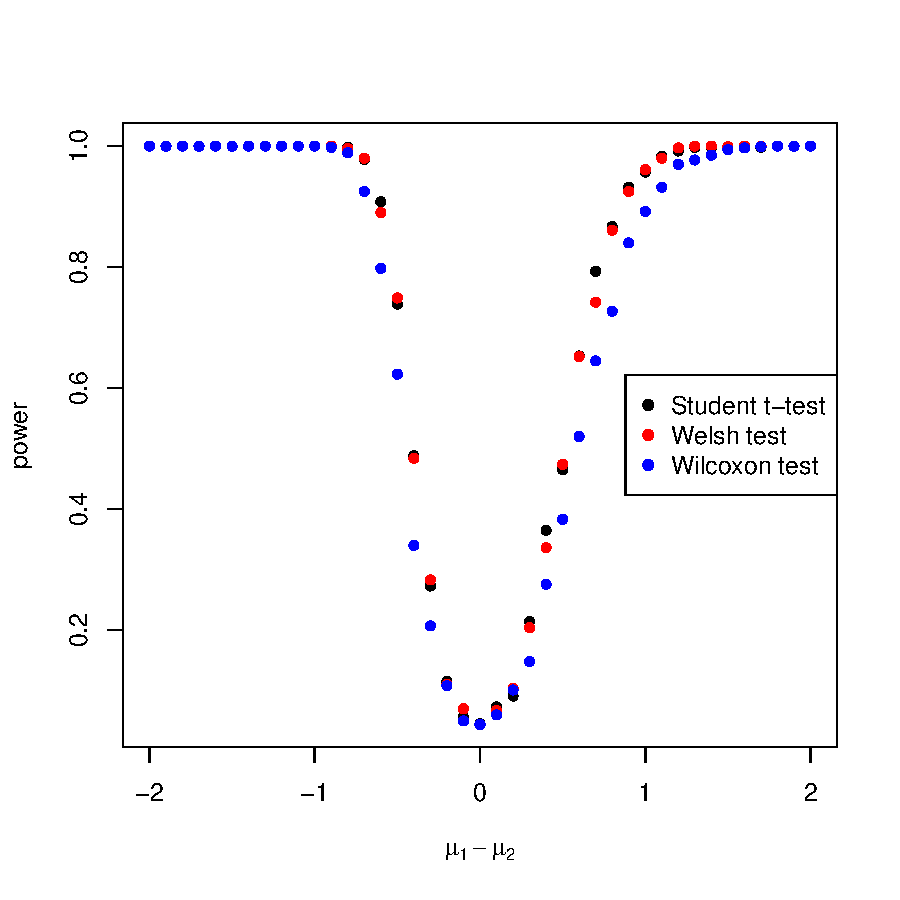
\includegraphics{p1-task_3_plot}
\label{chart_t3}
\caption{Power functions of three tests. Tests for two samples with exponential distribution}
\end{figure}

In the last task, we consider the non-normal distributions of samples. Thus the assumption for Student t-test and Welsh test about normality is not met but we would like to drop this assumption to see the power function. On the figure \ref{chart_t3} we can see that the power of all three tests is similar but the Wilcoxon test has lower values on the interval $[0,1]$. Comparing to the two other tasks the slope of the curve in last one is much more similar to the first one. The last thing that could be seen on the \ref{chart_t3} is the small non-symmetry -- the right side of the curve increase slower than the left one. 

\section{Conclusions}
In our work, we considered three tests in which two of them are extensions of Student t-test. This extension is based on the assumptions that must be meet in Student t-test. The plots of power function do not show huge differences between them. It might be caused by the fact that our sample is relatively large. There is no uniformly strongest test at the specified significance level among them. However, the results show that even if we did not have the data in the form that we would like to have (for example with normal distribution) we could substitute the most known test by other and get the test with similar power.



\end{document}
